\subsection{Выборочные характеристики}

Изначально было сгенерировано две выборки объёмом 60 и 80 значений из нормально распределённых генеральных совокупностей с разными случайными значениями параметров математического ожидания и среднеквадратического отклонения. Их этих двух выборок была сформирована обобщённая выборка (объёмом 140 значений), которая была упорядочена по возрастанию её значений с помощью сортировки.

Вручную были получены основные выборочные характеристики. Коэффициент вариации составляет 385\%, что говорит о большом разбросе значений и, как следствие, о неднородности выборки. Коэффициент асимметрии достаточно близок к нулю, что говорит о не большом отклонении от пика распределения (математического ожидания). Коэффициент эксцесса показывает, что данное распределение обладает более пологим пиком, чем эмпирическое.

Сгенерированная выборка и полученные выборочные характеристики представлены в конце отчёта.

Было произведено разбиение размаха выборки на конечное число непересекающихся интервалов. Число интервалов разбиения, согласно постановке задачи, производилось по следующим величинам:

\begin{itemize}
	\item $r = 10$;
	\item $r = 20$;
	\item $r = 30$;
	\item $r = [ 1 + 3.2 \lg{n} ]$, где $n$ - объём выборки.
\end{itemize}

Таким образом, для каждого $r$ были построены:

\newpage
\begin{itemize}
	\item Гистограмма частот распределения;
	
	\begin{figure}[H]
		\begin{minipage}[H]{0.44\linewidth}
			\center{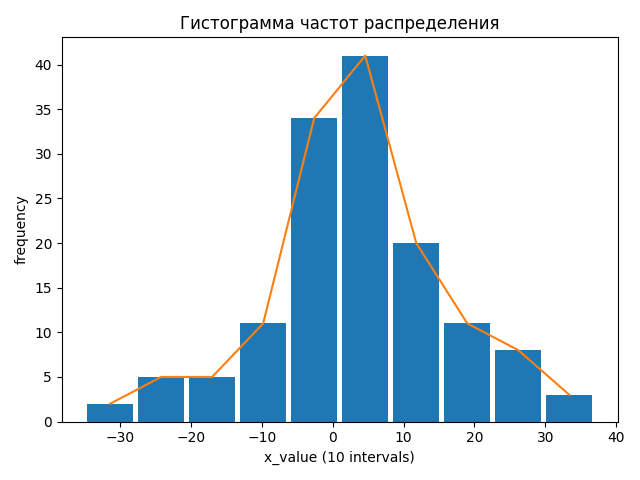
\includegraphics[width=\linewidth]{figures/freq_hist_10_bins}}
		\end{minipage}
		\hfill
		\begin{minipage}[H]{0.44\linewidth}
			\center{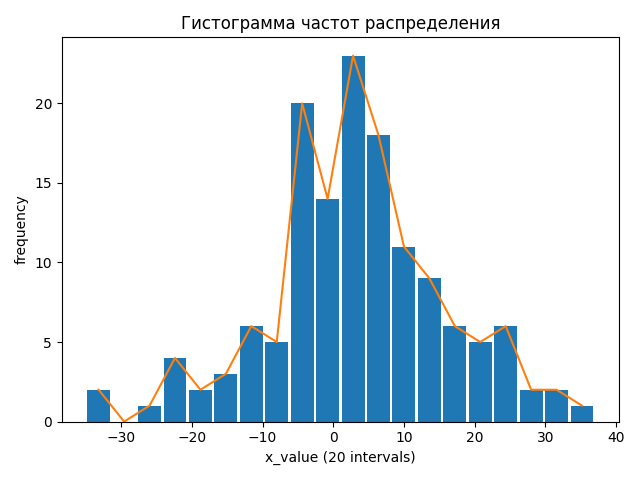
\includegraphics[width=\linewidth]{figures/freq_hist_20_bins}}
		\end{minipage}
		\vfill
		\begin{minipage}[H]{0.44\linewidth}
			\center{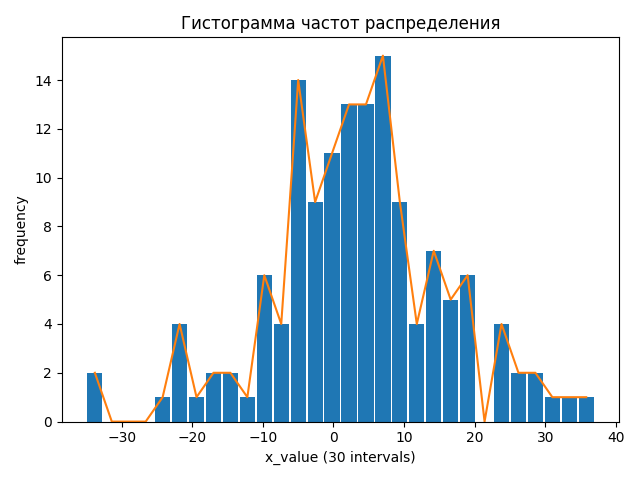
\includegraphics[width=\linewidth]{figures/freq_hist_30_bins}}
		\end{minipage}
		\hfill
		\begin{minipage}[H]{0.44\linewidth}
			\center{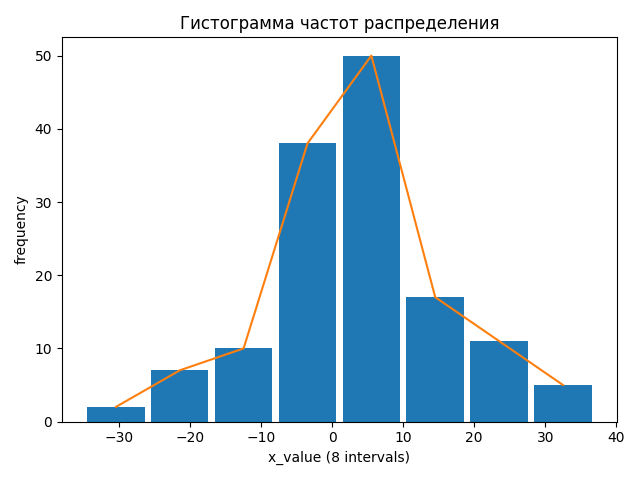
\includegraphics[width=\linewidth]{figures/freq_hist_8_bins}}
		\end{minipage}
	\end{figure}
	
	\item Гистограмма распределения частот и график интегральных частот;
	
	\begin{figure}[H]
		\begin{minipage}[H]{0.44\linewidth}
			\center{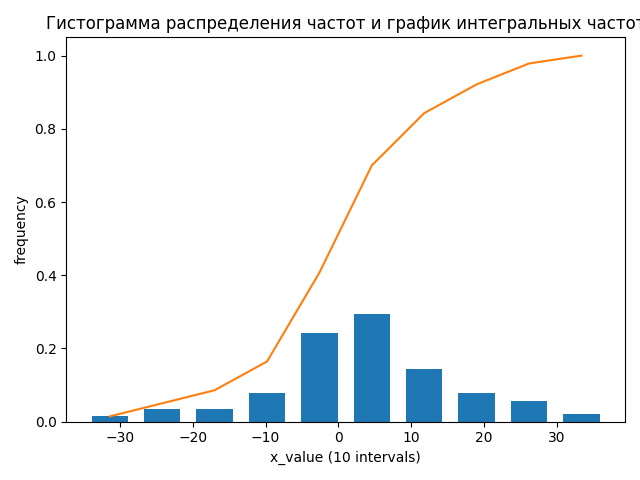
\includegraphics[width=\linewidth]{figures/freq_hist_cum_freq_10_bins}}
		\end{minipage}
		\hfill
		\begin{minipage}[H]{0.44\linewidth}
			\center{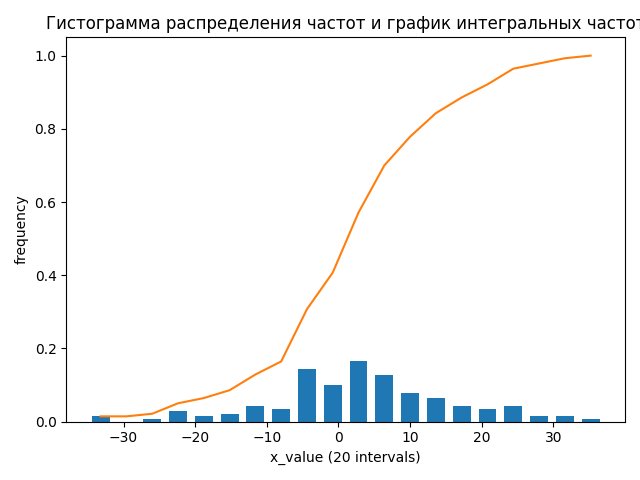
\includegraphics[width=\linewidth]{figures/freq_hist_cum_freq_20_bins}}
		\end{minipage}
		\vfill
		\begin{minipage}[H]{0.44\linewidth}
			\center{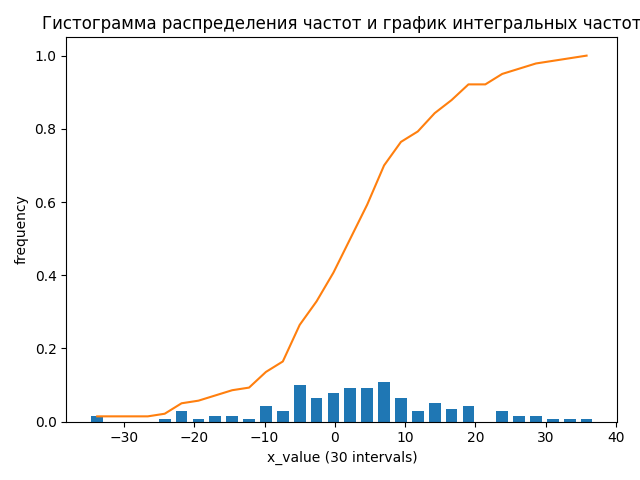
\includegraphics[width=\linewidth]{figures/freq_hist_cum_freq_30_bins}}
		\end{minipage}
		\hfill
		\begin{minipage}[H]{0.44\linewidth}
			\center{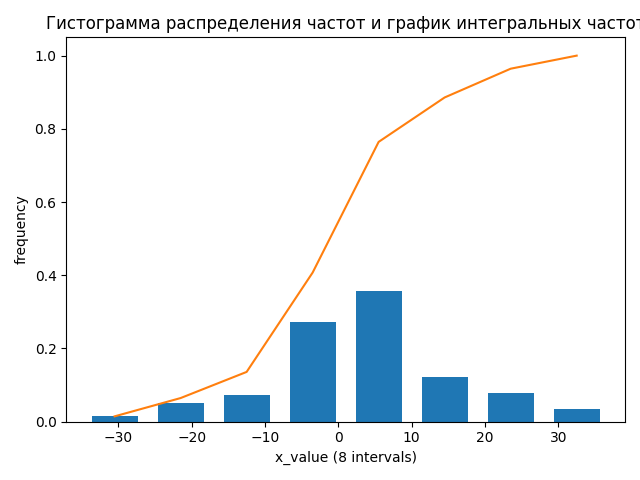
\includegraphics[width=\linewidth]{figures/freq_hist_cum_freq_8_bins}}
		\end{minipage}
	\end{figure}
	
	\item Гистограмма относительных кумулятивных частот;
	
	\begin{figure}[H]
		\begin{minipage}[H]{0.44\linewidth}
			\center{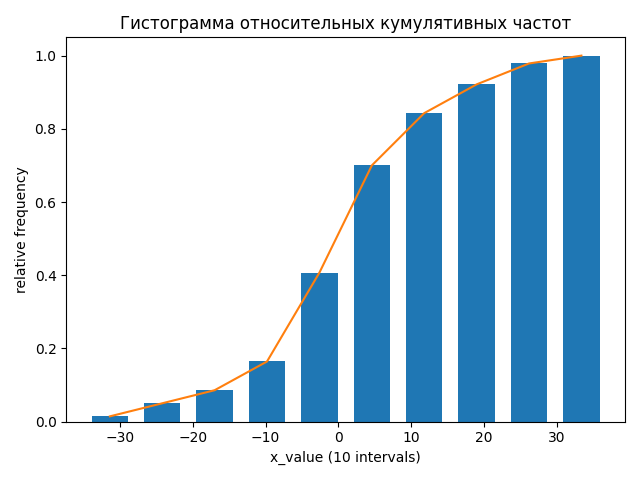
\includegraphics[width=\linewidth]{figures/rel_cum_hist_10_bins}}
		\end{minipage}
		\hfill
		\begin{minipage}[H]{0.44\linewidth}
			\center{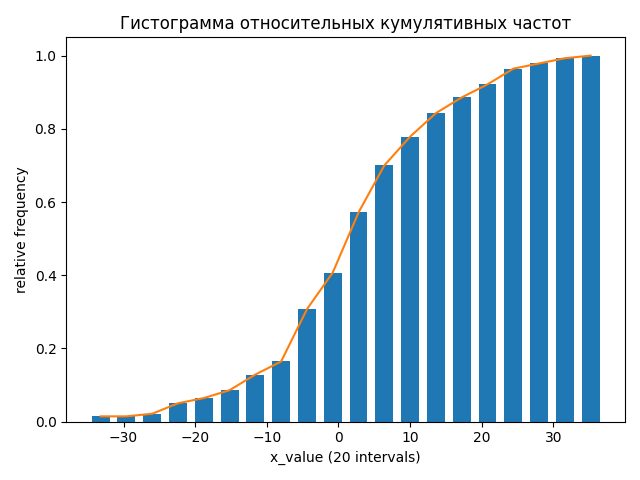
\includegraphics[width=\linewidth]{figures/rel_cum_hist_20_bins}}
		\end{minipage}
		\vfill
		\begin{minipage}[H]{0.44\linewidth}
			\center{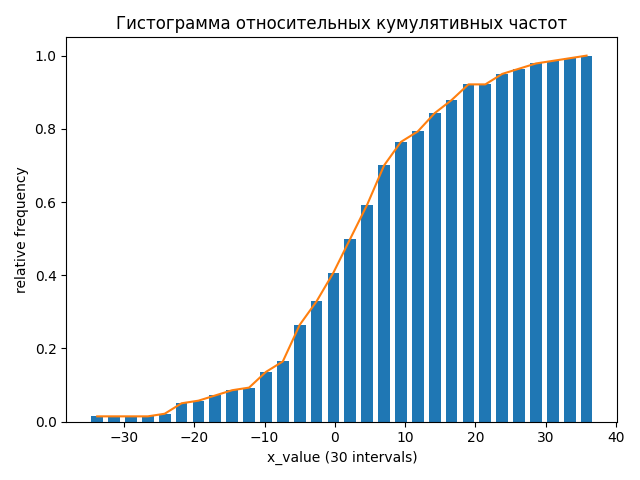
\includegraphics[width=\linewidth]{figures/rel_cum_hist_30_bins}}
		\end{minipage}
		\hfill
		\begin{minipage}[H]{0.44\linewidth}
			\center{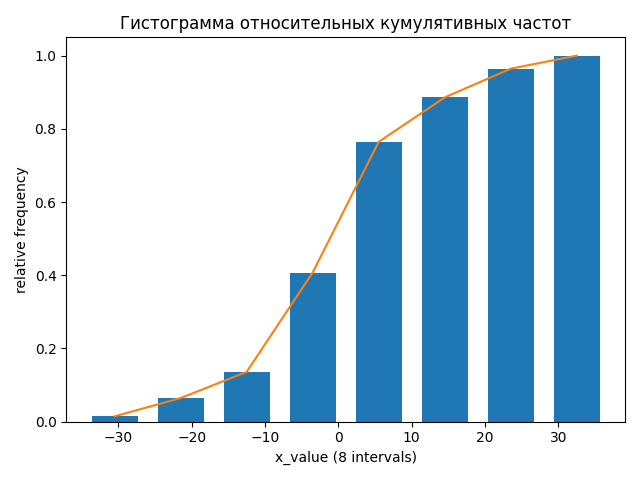
\includegraphics[width=\linewidth]{figures/rel_cum_hist_8_bins}}
		\end{minipage}
	\end{figure}
	
	\item Гистограмма плотности относительных частот;
	
	\begin{figure}[H]
		\begin{minipage}[H]{0.44\linewidth}
			\center{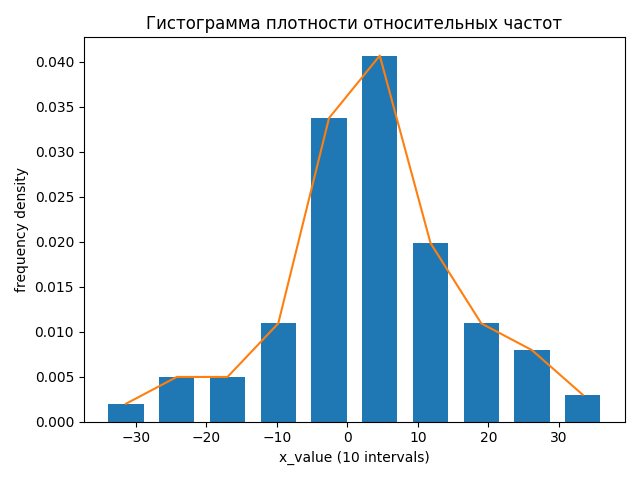
\includegraphics[width=\linewidth]{figures/rel_den_hist_10_bins}}
		\end{minipage}
		\hfill
		\begin{minipage}[H]{0.44\linewidth}
			\center{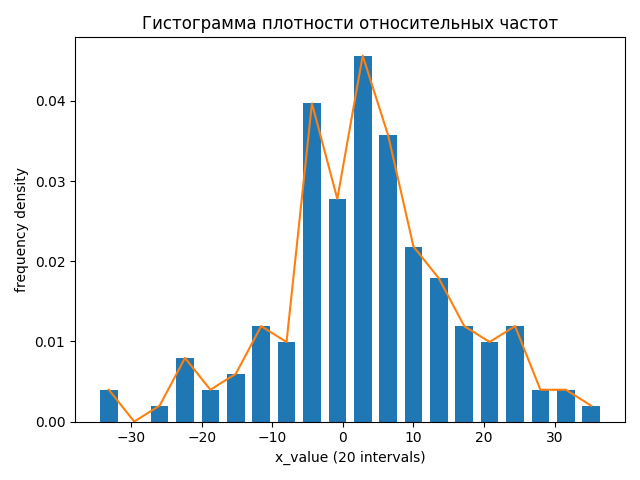
\includegraphics[width=\linewidth]{figures/rel_den_hist_20_bins}}
		\end{minipage}
		\vfill
		\begin{minipage}[H]{0.44\linewidth}
			\center{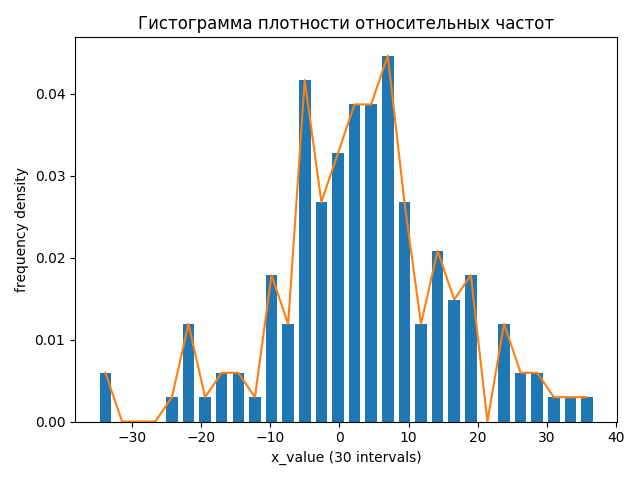
\includegraphics[width=\linewidth]{figures/rel_den_hist_30_bins}}
		\end{minipage}
		\hfill
		\begin{minipage}[H]{0.44\linewidth}
			\center{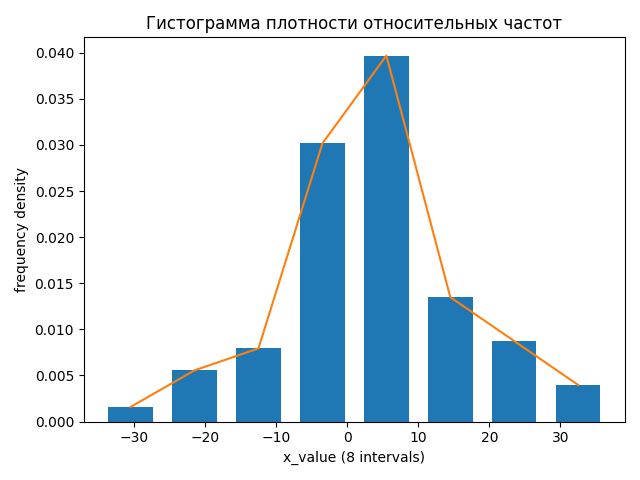
\includegraphics[width=\linewidth]{figures/rel_den_hist_8_bins}}
		\end{minipage}
	\end{figure}
	
	\item Гистограмма относительных частот.
	
	\begin{figure}[H]
		\begin{minipage}[H]{0.44\linewidth}
			\center{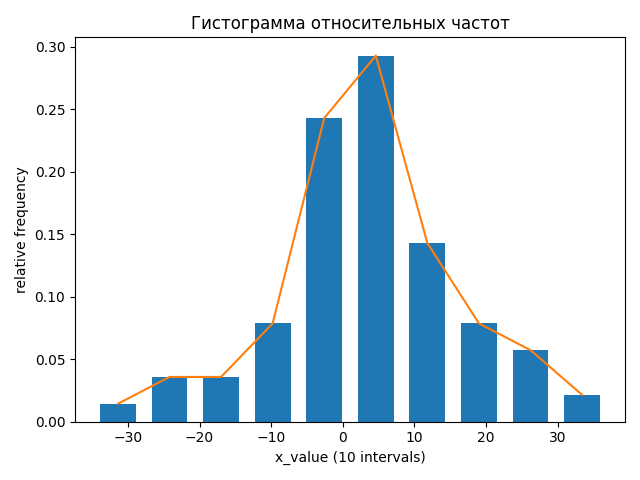
\includegraphics[width=\linewidth]{figures/rel_freq_hist_10_bins}}
		\end{minipage}
		\hfill
		\begin{minipage}[H]{0.44\linewidth}
			\center{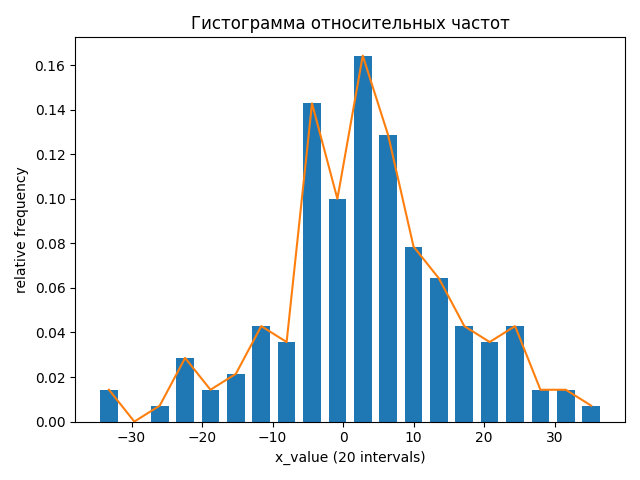
\includegraphics[width=\linewidth]{figures/rel_freq_hist_20_bins}}
		\end{minipage}
		\vfill
		\begin{minipage}[H]{0.44\linewidth}
			\center{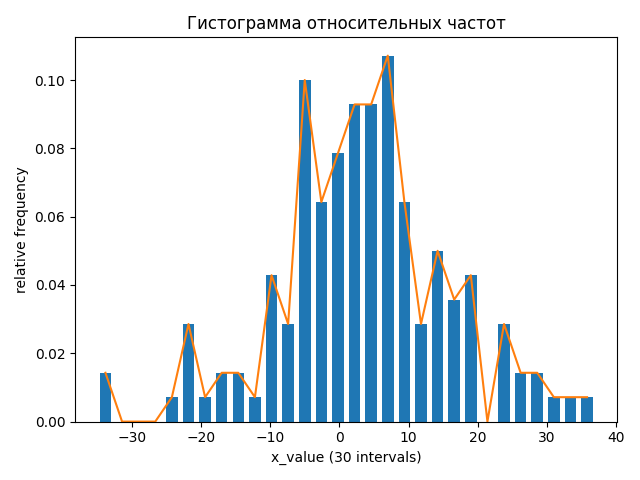
\includegraphics[width=\linewidth]{figures/rel_freq_hist_30_bins}}
		\end{minipage}
		\hfill
		\begin{minipage}[H]{0.44\linewidth}
			\center{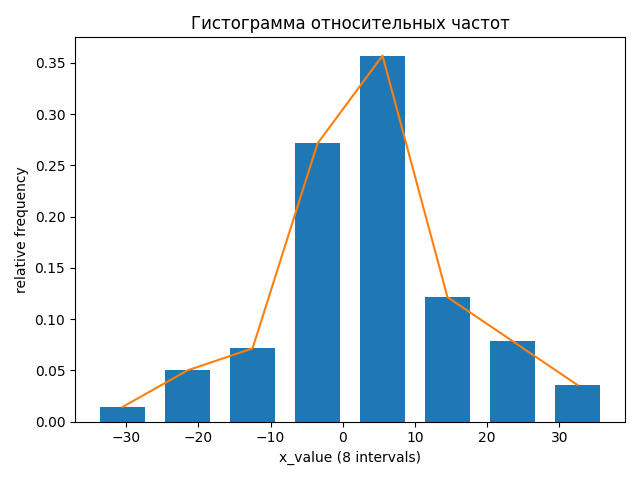
\includegraphics[width=\linewidth]{figures/rel_freq_hist_8_bins}}
		\end{minipage}
	\end{figure}
	
\end{itemize}

При малых интервалах разбиения ($r = 8, r = 10 $) нельзя утверждать о неоднородности выборки, однако при увеличении числа интервалов становится явно видно 2 пика, которые и могут послужить аргументом для утверждения неоднородности выборки. Исходя из дескриптивной статистики, можно также сделать вывод о наличии существенной неоднородности в исходных данных.

Таким образом, в ходе работы были вычислены основные статистические характеристики, построены гистограммы, полигоны плотности и кумулятивные частоты и на основе всего вышеперечисленного сделаны выводы.
